\section{Discussion}
\label{sec:summary-discussion}

Are there any objects that might not be bow shocks?

Progression in density:
\begin{gather*}
  \text{Increasing density} \longrightarrow \\
  \text{WBS} \to \text{WBS} + \text{IDW} \to \text{WBS} + \text{DDW} \to \text{(RBW)} \to \text{RBS}
\end{gather*}

Chief diagnostic for radiation supported bows (RBW or RBS cases) is
infrared luminosity of bow.  Favored by high densities.

Dust waves favored by high velocities and intermediate densities.


\subsection{$\sigma$ Ori as a dust wave candidate}
\label{sec:sigma-ori-as}

\begin{figure}
  \centering
  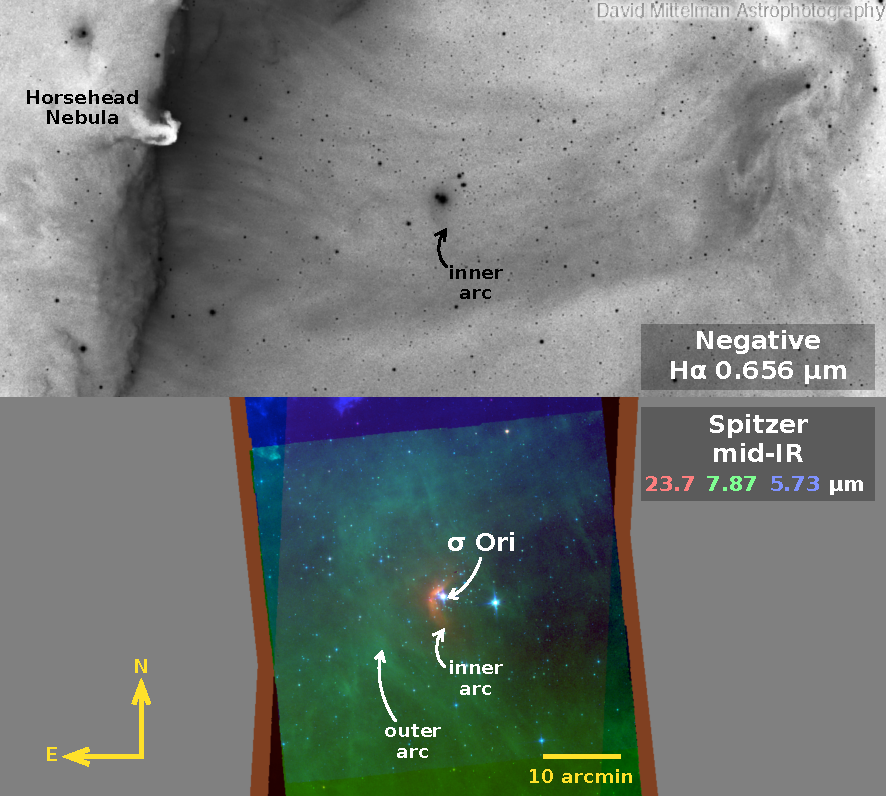
\includegraphics[width=\linewidth]{figs/sigma-ori-comparison}
  \caption{Optical and infrared images of $\sigma$~Ori}
  \label{fig:sig-ori}
\end{figure}

\begin{figure}
  \centering
  \includegraphics[width=\linewidth]{figs/sigma-ori-eastwest-cuts}
  \caption{Brightness profiles through $\sigma$~Ori inner arc.}
  \label{fig:sig-ori-cuts}
\end{figure}





How different regions of the \(\Pi\)--\(\Lambda\) plane are populated.
Bottom-right quadrant hard to get to (except for standing wave
oscillations), but may be due to finite shell thickness, which (for
low Mach number) will be more apparent in the wings, which might
decrease \(\Lambda\) more than \(\Pi\).  Fact that thin-shell solutions should
trace the contact discontinuity, but in some cases it may be only the
inner or the outer shell that is visible.

Justification for standing waves: Fig.~3 of \citet{Meyer:2016a} shows
a time sequence of thin-shell instability, which looks a bit like a
standing wave. But much larger amplitude than we are considering.

Deviations from axisymmetry as an alternative to oscillations. 


\subsection{The case of inside-out bows}
\label{sec:case-inside-out}

So far, we have considered the case where the inner source dominates
the radiation, while dust is present only in the outer stream, which
applies to hot stars interacting with the ISM.  However, in the case
of cool stars, the inner wind will also be dusty.  Examples are the
red supergiant (RSG) phase of high-mass evolution, or the asymptotic
giant branch (AGB) stage of low/intermediate-mass evolution.  In both
these cases, it is still the inner source that provides the radiation
field.  However, not all winds are radiatively driven and in those
cases it is conceivable that it is the outer source that dominates the
radiation field.  An example is the case of photoevaporating
protoplanetary disks (proplyds) in the Orion Nebula and other \hii{}
regions \citep{ODell:1994a}.  In the proplyds, the inner wind is a
thermally driven photoevaporation flow \citep{HA:1998, Henney:1999a},
while the outer stream is the stellar wind from an O~star
\citep{Garcia-Arredondo:2001a}.


\section{Summary and conclusions}
\label{sec:conclusions}



%%% Local Variables:
%%% mode: latex
%%% TeX-master: "dusty-bow-wave"
%%% End:
